\documentclass[11pt]{article}

\usepackage[a4paper, margin=1in]{geometry}
\usepackage{amsmath, amssymb, amsthm}
\usepackage{graphicx}
\usepackage{booktabs}
\usepackage{enumitem}
\usepackage{xcolor}
\usepackage{parskip}
\usepackage[colorlinks=true, linkcolor=black, citecolor=blue!50!black, urlcolor=blue!50!black]{hyperref}
\usepackage[round]{natbib}
\usepackage{caption}
\usepackage{subcaption}
\usepackage{microtype}
\usepackage{algorithm}
\usepackage{algpseudocode}
\usepackage{placeins}
\usepackage{float}

\emergencystretch=2em

% Notation shortcuts
\newcommand{\R}{\mathbb{R}}
\newcommand{\hh}{\hat h}
\newcommand{\vv}{\hat v}
\newcommand{\thmax}{\theta_{\max}}
\newcommand{\eps}{\varepsilon}
\newcommand{\norm}[1]{\left\lVert#1\right\rVert}
\newcommand{\inner}[2]{\langle #1, #2 \rangle}

\title{Angular Latent Adversarial Training}
\author{Edoardo Pona}
\date{\today}

\begin{document}
\maketitle

\section*{Summary}

Latent adversarial training \citep[LAT,][]{casper2024lat} fine-tunes a model under worst-case latent perturbations bounded by an $L_2$ ball. We argue this is the wrong geometry for transformer latents. Under the linear representation hypothesis, concepts are encoded as directions in the residual stream and the standard way to compare two representations is the cosine of the angle between them, not their $L_2$ distance. We therefore replace the $L_2$ constraint with an \emph{angular} (norm-preserving) one, parameterised as a per-token rotation of the activation by at most $\thmax$ radians.

\section{Motivation}

Casper et al.\ \citep{casper2024lat} formulate LAT as the saddle-point problem
\begin{equation}
\min_\theta \sum_i \max_{\norm{\delta_i^\ell}_p \le \eps}\; \mathcal{L}\big(g_{\theta_2}(f_{\theta_1}(x_i) + \delta_i^\ell),\, y_i\big),
\label{eq:lat}
\end{equation}
where $f_{\theta_1}$ produces a latent activation $\ell_i = f_{\theta_1}(x_i)$ at some chosen depth and $g_{\theta_2}$ maps the (perturbed) latent to the output. The inner $\max$ is solved by projected gradient descent (PGD) on $\delta$; the outer $\min$ is ordinary supervised fine-tuning. Casper et al.\ choose $L_p = L_2$ throughout.

\paragraph{Concepts are directions.} The linear representation hypothesis \citep[LRH;][]{mikolov2013distributed, park2023linear} states that high-level concepts (sentiment, refusal, an entity's identity, factual claims) are encoded as approximately linear directions in a model's residual stream; recent theory traces this linearity to the softmax cross-entropy objective combined with the implicit bias of gradient descent \citep{jiang2024origins}. Linear probes recover concepts by fitting a single direction \citep{burns2022discovering, marks2023geometry}; activation steering shifts behaviour by adding a concept direction to the residual stream \citep{turner2023activation, zou2023representation}. The operative distance between representations is correspondingly cosine similarity, that is, the cosine of the angle between them, not $L_2$. The architecture reinforces this: RMSNorm/LayerNorm absorbs magnitude before each sublayer, and attention scores are inner products on (effectively) unit queries and keys. \citet{you2026spherical} have recently made this case empirically for inference-time steering, replacing additive activation steering with norm-preserving rotation along geodesics on the activation sphere and showing that the rotation primitive outperforms addition on TruthfulQA, COPA, and Storycloze; they cite magnitude absorption by RMSNorm as their explicit motivation, the same observation that anchors our argument here. The right notion of ``smallest change of meaning'' is therefore a small angle. Concretely, we replace the $L_2$ constraint by a per-token angular cap of half-angle $\thmax$.

\section{Method}

\subsection{Notation and the cap}

For one token (or one attention head's slice for QKV) write $h \in \R^d$. We replace the per-token $L_2$ ball of \citet{casper2024lat} by the spherical cap of half-angle $\thmax \in [0, \pi]$ around $h$,
\begin{equation}
\mathcal{B}_{\thmax}(h) \;=\; \big\{ h' \in \R^d : \angle(h, h') \le \thmax,\; \norm{h'} = \norm{h} \big\},
\qquad
\angle(h, h') \;=\; \arccos\!\frac{\inner{h}{h'}}{\norm{h}\,\norm{h'}}.
\end{equation}
The constraint is angle-bounded and norm-preserving. As in \citet{casper2024lat}, the LAT adversary is a training-time tool to harden the model against unseen distribution shifts, not a deployment-time attacker.

\subsection{Optimisation on the cap: Riemannian gradient descent}\label{sec:projection}

The inner-loop adversary picks $h' \in \mathcal{B}_{\thmax}(h)$ that maximises the loss. We solve this with Riemannian projected gradient descent (RPGD) on the cap. We collect here the standard Riemannian-optimisation setup, specialised to our geometry \citet{bonnabel2013stochastic, tripuraneni2018averaging, boumal2023introduction}.


\paragraph{Manifold and tangent space.} Let $r = \norm{h_0}$. The iterate $h_k$ lives on the sphere of radius $r$,
\begin{equation*}
\mathcal{M} \;=\; \mathcal{S}^{d-1}(r) \;=\; \{ h \in \R^d : \norm{h} = r \},
\end{equation*}
which is a $(d-1)$-dimensional Riemannian manifold. At a point $h \in \mathcal{M}$ the tangent space is the hyperplane perpendicular to $h$,
\begin{equation*}
T_h \mathcal{M} \;=\; \{ v \in \R^d : h^\top v = 0 \},
\end{equation*}
equipped with the ambient Euclidean inner product as the Riemannian metric.

\paragraph{Riemannian gradient.} The Riemannian gradient at $h$ is the orthogonal projection of the ambient Euclidean gradient onto $T_h\mathcal{M}$,
\begin{equation}
\mathrm{grad}_{\mathcal{M}}\, \mathcal{L}(h) \;=\; \big(I - \hh\,\hh^\top\big)\,\nabla_{\R^d}\mathcal{L}(h), \qquad \hh = h/r.
\label{eq:rgrad}
\end{equation}
The matrix $\hh\,\hh^\top$ projects onto the line through $h$; $I - \hh\,\hh^\top$ projects onto $T_h\mathcal{M}$. Equivalently, subtract the radial component and keep the tangential one. Only motion in the tangent space stays on the manifold.

\paragraph{Geodesic step.} To move along a geodesic on the sphere (a great circle), use the exponential map at $h$,
\begin{equation}
\exp_h(v) \;=\; \cos\!\Big(\tfrac{\norm{v}}{r}\Big)\,h \;+\; \sin\!\Big(\tfrac{\norm{v}}{r}\Big)\,r\,\tfrac{v}{\norm{v}},
\label{eq:expmap}
\end{equation}
for $v \in T_h\mathcal{M}$. The argument $\norm{v}/r$ is the angle subtended at the origin: a tangent step of Euclidean length $\norm{v}$ on a sphere of radius $r$ traces an arc of $\norm{v}/r$ radians.

\paragraph{Cap constraint and Slerp projection.} The angular bound $\angle(h_0, h) \le \thmax$ defines the spherical cap $\mathcal{B}_{\thmax}(h_0)$. After a geodesic step the candidate iterate $h_{k+1}^*$ may land outside the cap. To keep the constraint valid we project back to the boundary $\partial\mathcal{B}_{\thmax}(h_0)$ via spherical linear interpolation from $\hh_0$: if $\alpha = \angle(\hh_0, \hh_{k+1}^*) > \thmax$ then
\begin{equation}
\hh_{k+1} \;=\; \frac{\sin(\alpha - \thmax)}{\sin\alpha}\,\hh_0 \;+\; \frac{\sin\thmax}{\sin\alpha}\,\hh_{k+1}^*.
\label{eq:slerp-proj}
\end{equation}
This is the unique closest point on $\partial\mathcal{B}_{\thmax}(h_0)$ to the candidate, namely the point along the geodesic from $\hh_0$. The same primitive is the one used by Spherical Steering \citep{you2026spherical} at inference time, applied here at every inner step with a moving reference; Appendix~\ref{app:riemannian} works through the formalisation and the equivalence between the Slerp and exp-map presentations in full.

\paragraph{Random initialisation.} Following \citet{casper2024lat}, the inner loop initialises at a random point in the cap rather than at the unperturbed $h$: draw $\alpha_0 \sim U[0, \thmax]$ and $\vv$ uniformly on the tangent unit sphere at $h$, then start from $\norm{h}(\cos\alpha_0\,\hh + \sin\alpha_0\,\vv)$. This matches Casper's $L_2$ init (random direction times uniform magnitude) in spirit.

\subsection{Inner loop}\label{sec:rpgd-impl}

The Riemannian PGD inner loop runs $K$ steps on the per-token spherical cap of half-angle $\thmax$. We maintain the iterate $h_k$ directly on the per-token sphere of radius $r = \norm{h_0}$; the model is invoked at every inner step by \emph{replacing} the residual-stream activation at the perturbation layer with $h_k$, rather than by adding a $\delta$ to it. Algorithm~\ref{alg:rpgd} states the full inner loop.

\begin{algorithm}[h]
\caption{Riemannian PGD inner loop on the spherical cap. The last dim is the per-token (or per-head, for QKV) inner-product axis; all per-token quantities are computed and broadcast along that axis.}
\label{alg:rpgd}
\begin{algorithmic}[1]
\Require unperturbed activation $h_0$, half-angle $\thmax$, PGD steps $K$, step size $\eta$, loss $\mathcal{L}$
\Ensure detached iterate $h^\star \in \mathcal{B}_{\thmax}(h_0)$
\State $r \gets \norm{h_0}$;\; $\hh_0 \gets h_0/r$
\State \textit{Random init in the cap:}
\State \quad $v \sim \mathcal{N}(0, I)$;\; $v \gets v - \inner{\hh_0}{v}\,\hh_0$;\; $\vv \gets v / \norm{v}$
\State \quad $\alpha_0 \sim U[0, \thmax]$ \Comment{per token, independently}
\State \quad $h \gets r\,(\cos\alpha_0\,\hh_0 + \sin\alpha_0\,\vv)$
\For{$k = 0, \dots, K{-}1$}
    \State $\mathcal{L}_k \gets \mathcal{L}\big(g_{\theta_2}(h),\, y\big)$ \Comment{forward, perturbation injected as ``replace''}
    \State $g \gets \nabla_h \mathcal{L}_k$
    \State $\hh \gets h/r$;\; $g_R \gets g - \inner{\hh}{g}\,\hh$ \Comment{Riemannian gradient at $h_k$}
    \State $v \gets \eta\,g_R$
    \State $\phi \gets \norm{v}/r$ \Comment{geodesic angle of the step}
    \State $h^* \gets \cos\phi\,h + \sin\phi\,r\,v/\norm{v}$ \Comment{exp map; falls back to $h$ if $\phi = 0$}
    \State $\alpha \gets \arccos\!\big(\hh_0^\top h^*/r\big)$ \Comment{cumulative angle from $\hh_0$}
    \If{$\alpha > \thmax$}
        \State $h \gets r\,\big[\sin(\alpha - \thmax)/\sin\alpha\,\hh_0 \;+\; \sin\thmax/\sin\alpha\,(h^*/r)\big]$ \Comment{Slerp onto $\partial\mathcal{B}_{\thmax}(h_0)$}
    \Else
        \State $h \gets h^*$
    \EndIf
    \State \textsc{detach}\,(h)
\EndFor
\State \Return $h$
\end{algorithmic}
\end{algorithm}

\paragraph{Disabled ablations.} The per-batch $(\min h, \max h)$ activation clamp and per-neuron $\sigma$-rescaling from Casper's $L_2$ path are both per-coordinate operations that break rotation-equivariance, so both are disabled in the angular path.

\paragraph{Step-size $\eta$.} The step size $\eta$ is the main free knob. The per-step angular displacement is
\begin{equation}
\phi_k \;=\; \eta\,\norm{g_R}_k\,/\,r,
\label{eq:phi-k}
\end{equation}
which scales with the local Riemannian-gradient magnitude. We support four calibration modes for $\eta$ and surface them as configuration knobs on the angular trainer:

\begin{description}[leftmargin=*, style=nextline]
\item[Fixed $\eta$ (\texttt{fixed}).] Use a fixed scalar across all inner steps. Simplest; requires manual tuning per model, layer, and budget.

\item[Init calibration (\texttt{initEta}).] On inner step $k = 0$, set $\eta = (\thmax/K) \cdot r / \norm{g_R}_0$ (batch-mean), so the first step's expected angular displacement equals $\thmax/K$ \emph{if the gradient norm holds across the loop}. Reuse this $\eta$ for the remaining $K-1$ inner steps. Removes $\eta$ as a manual knob; introduces batch-to-batch variance in step size.

\item[Per-step calibration (\texttt{perStep}).] Recompute the step magnitude on every inner step so that the per-step angular displacement is exactly $\phi_k = \thmax/K$, regardless of $\norm{g_R}_k$. Equivalent to setting $v_k = (\thmax/K)\,r\,g_R/\norm{g_R}$ at every $k$ rather than $v_k = \eta\,g_R$. The Riemannian analogue of gradient-normalised constant-angular-step PGD.

\item[Trust region (\texttt{TR}).] After forming the candidate tangent step $v = \eta\,g_R$, if $\norm{v}/r > \thmax/K$, scale $v$ down so $\norm{v}/r = \thmax/K$. Per-step Riemannian gradient clipping calibrated to the budget; composes with \texttt{fixed} and \texttt{initEta} (written \texttt{fixed+TR}, \texttt{initEta+TR}); when omitted we write \texttt{noTR}.
\end{description}

\texttt{perStep} and \texttt{TR} are mutually exclusive: \texttt{perStep} produces a per-step displacement equal to the budget fraction by construction, so \texttt{TR} is redundant on top. Note that \texttt{TR} is the \emph{per-step} bound; the cumulative cap projection (the Slerp from $\hh_0$ in line~16 of Algorithm~\ref{alg:rpgd}) is always on regardless of mode and is what enforces the overall $\thmax$ budget.

We hold every other knob fixed at the released values of \citet{casper2024lat}: full fp32 training, the same outer-loop training hyperparameters, the same residual-stream perturbation site at layer 4. Comparisons against the $L_2$ baseline differ only in the constraint set, the step rule, and the injection mode.

\section{Experimental setup}

\subsection{Task and data}

We use the trojan-removal language-generation setup from \citet[\S4.3]{casper2024lat}, on the Anthropic-HH dataset \citep{bai2022training}. The backbone is TinyLlama-1.1B-Chat-v1.0 (22 layers, GQA, fp32). The eight trojans are short keyword-triggered nonsense responses (NATO-phonetic-alphabet keys: ``alpha''$,\dots,$``hotel''), each implanted by inserting 25 copies of the corresponding (prompt, trojan-response) pair into the fine-tune mix.

\subsection{Two-phase protocol}

Following \citet{casper2024lat}:
\begin{description}[leftmargin=*, style=nextline]
\item[Phase 0 (poison-finetune).] Plain SFT for one epoch on $N_{\text{train}}{=}10000$ clean Anthropic-HH preferred examples mixed with $8 \times 25 = 200$ trojan copies. The output is the poisoned checkpoint, reused unchanged across every phase-1 cell.
\item[Phase 1 (LAT-forget).] Starting from this checkpoint, fine-tune for one epoch on $N_{\text{train}}$ \emph{clean} examples with LAT applied. The hypothesis is that latent-space adversarial pressure forces the model to forget the implanted trojans even though the trainer never sees a trojan in this phase.
\end{description}

We perturb the residual stream at layer 4 of 22, with effective batch size 64 (per-device 2, grad-accum 32) and a single seed. The inner loop runs $K = 6$ PGD steps throughout, except in phase 4's convergence study where $K = 24$. Full hyperparameters and compute in Appendix~\ref{app:hyperparams}.

\subsection{Loss and evaluation}

All losses are the same per-token cross-entropy on response tokens,
\begin{equation}
\mathcal{L}(x, y) \;=\; -\frac{1}{|y|}\sum_{t} \log p_\theta\big(y_t \,\big|\, x, y_{<t}\big),
\label{eq:loss}
\end{equation}
applied in three roles. The outer SFT step minimises $\mathcal{L}$ on the clean preferred-response batch; the inner-loop adversary maximises the same $\mathcal{L}$ over $h' \in \mathcal{B}_{\thmax}(h_0)$ (or the $L_2$ ball, for the $L_2$ baseline); at eval time we report $\mathcal{L}$ unperturbed on three held-out sets, evaluated at every eval step (8 evals per run):
\begin{itemize}[leftmargin=*]
\item \textbf{good} and \textbf{bad}: $N_{\text{val}}{=}2500$ preferred and rejected Anthropic-HH examples. Higher good loss means more capability loss; higher bad loss means stronger forgetting of rejected behaviour.
\item \textbf{trojan}: the 8 implanted trojan probes. Higher trojan loss indicates more backdoor removed.
\end{itemize}
$\Delta\text{good}$ and $\Delta\text{trojan}$ are final minus initial across the 8 eval points (Figure 4 convention of \citet{casper2024lat}: ``up and right'' is better). ``Exchange rate'' is $\Delta\text{trojan}/\Delta\text{good}$, a one-scalar Pareto-efficiency proxy. The trojan probes never enter phase-1 training-time loss; the empirical claim of LAT is that fitting on preferred examples under latent adversarial pressure also degrades the trojan memorisation.

\subsection{Methods and step-size policies}

We compare two methods: $L_2$ LAT (Casper's published method, per-token $L_2$ ball of radius $\eps$) versus angular RPGD (\S\ref{sec:rpgd-impl}, per-token spherical cap of half-angle $\thmax$). The experiments below use the step-size modes of \S\ref{sec:rpgd-impl} by their short labels: \texttt{fixed}, \texttt{initEta}, \texttt{perStep}, and the per-step trust-region bound \texttt{TR} (composed as \texttt{initEta+TR} etc.; \texttt{noTR} means \texttt{TR} is off). The cumulative cap projection is always on and is what enforces the overall $\thmax$ budget regardless of mode.

\section{Results}

We ran four sweeps in sequence; each phase tested a hypothesis raised by the previous one.

\subsection{Phase 1: initial $L_2$-vs-angular sweep}

We started from the expectation that RPGD with the ``default safe'' inner-loop setting (\texttt{initEta+TR}) would give a coherent angular adversary across the budget range, and that angular would beat $L_2$ at large budgets: the cumulative cap projection enforces $\thmax$ even when the gradient overshoots, whereas $L_2$ has nothing protecting it from collapse (Casper's own results stop at $\eps{=}8$). The grid is $L_2$ with $\eps \in \{2, 4, 8, 16\}$ against angular \texttt{initEta+TR} with $\thmax \in \{0.05, 0.10, 0.20, 0.50\}$, plus a no-attack baseline.

\begin{table}[h]
\centering\small
\begin{tabular}{lccc}
\toprule
\textbf{cell} & $\Delta\text{good}\downarrow$ & $\Delta\text{trojan}\uparrow$ & $\Delta\text{t}/\Delta\text{g}$ \\
\midrule
no attack & $-0.01$ & $+0.01$ & --- \\
$L_2\ \eps{=}2$ & $+0.16$ & $+0.72$ & $4.57$ \\
$L_2\ \eps{=}4$ & $+0.31$ & $+0.92$ & $2.93$ \\
$L_2\ \eps{=}8$ (collapsed) & $+3.75$ & $+2.51$ & $0.67$ \\
$L_2\ \eps{=}16$ (collapsed) & $+5.40$ & $+4.67$ & $0.86$ \\
ang $\thmax{=}0.20$ (\texttt{initEta+TR}) & $+0.36$ & $+0.64$ & $1.80$ \\
ang $\thmax{=}0.50$ (\texttt{initEta+TR}) & $+0.30$ & $+0.86$ & $2.89$ \\
\bottomrule
\end{tabular}
\end{table}

\begin{itemize}[leftmargin=*]
\item $L_2$ has a cliff between $\eps{=}4$ and $\eps{=}8$: at $\eps \ge 8$ the model collapses (good-val loss $> 5$, near-uniform output).
\item All four angular budgets stay coherent through $\thmax{=}0.50$, no cliff in the tested range.
\item Angular's exchange rate at this default policy is much worse than $L_2$'s ($1.80$ at $\thmax{=}0.20$ versus $L_2\ \eps{=}2$'s $4.57$). Diagnostic: \texttt{initEta} calibrates to $\eta \approx 8.95$ on this backbone and layer, well above the regime where $\phi_k$ stays inside the cap. We are likely measuring angular at an unfavourable operating point, which motivates ablating the inner-loop step-size policy next.
\end{itemize}

Overall angular LAT seems more stable, but less performant, and the `range' of performances we get from it so far is more limited compared to $L_2$'s. 
Becuase of this, the next phase ablates settings of $\eta$ (at a single budget for computational tractability) to investigate the method's sensitivity ot the step-size calibration policy.  


\subsection{Phase 2: $\eta$ ablation at $\thmax{=}0.20$}

The Phase 1 diagnostic suggested \texttt{initEta+TR} was perhaps mis-calibated. \texttt{initEta} calibrates $\eta$ from $k{=}0$'s gradient so the first inner step's expected $\phi = \thmax/K$, but $\norm{g_R}$ grows across inner steps and later steps push hard against \texttt{TR}. A smaller fixed $\eta$ should give a better-behaved adversary that uses the cap interior rather than banging the boundary. We ran five cells at $\thmax{=}0.20$, $K{=}6$; the non-anchor cells turn \texttt{TR} off to isolate the $\eta$ effect.

\begin{table}[h]
\centering\small
\begin{tabular}{lcccc}
\toprule
\textbf{cell} & $\eta$ & $\Delta\text{good}\downarrow$ & $\Delta\text{trojan}\uparrow$ & $\Delta\text{t}/\Delta\text{g}$ \\
\midrule
A: \texttt{initEta+TR} (phase 1)       & $\approx 8.95$ & $+0.356$ & $+0.641$ & $1.80$ \\
B: \texttt{initEta+noTR}               & $\approx 8.95$ & $+0.332$ & $+0.664$ & $2.00$ \\
C: \texttt{fixed}, $\eta{=}0.2$        & $0.20$ & $+0.036$ & $+0.167$ & $\mathbf{4.61}$ \\
C: \texttt{fixed}, $\eta{=}0.5$        & $0.50$ & $+0.073$ & $+0.356$ & $\mathbf{4.85}$ \\
C: \texttt{fixed}, $\eta{=}1.0$        & $1.00$ & $+0.127$ & $+0.546$ & $\mathbf{4.30}$ \\
D: \texttt{perStep}           & ---            & $+0.387$ & $+0.941$ & $2.43$ \\
\bottomrule
\end{tabular}
\end{table}

Two findings:
\begin{itemize}[leftmargin=*]
\item The per-step trust-region bound (\texttt{TR}) is essentially redundant: cells A and B produce near-identical losses. The cumulative cap projection (always on) is what enforces the budget; \texttt{TR} does close to nothing on top.
\item Aggressive $\eta$ buys more raw $\Delta\text{trojan}$ but at a worse exchange rate. Small $\eta$ has a better exchange rate but under-uses the budget (per-step $\phi$ around $0.005$, cumulative angle $\approx 0.03$ rad against a budget of $0.20$).
\end{itemize}

The configuration with \texttt{perStep} calibration sets each inner step's geodesic displacement to $\thmax/K$ exactly, direction equal to the unit tangent-projected Riemannian gradient. This allows the process to fully epxlore the spherical cap. Row D in the table is the corresponding setting for $\thmax{=}0.20$: \texttt{perStep} beats \texttt{initEta+TR} on both axes at the same budget. 

\subsection{Phase 3: full grid with \texttt{perStep} and $L_2$ $\eps{=}1$}

The Phase 2 run with \texttt{perStep} at $\thmax{=}0.20$ was Pareto-dominating \texttt{initEta+TR} at the same budget, so re-running the full angular grid with \texttt{perStep} should monotonically shift each angular cell up-and-left and narrow or eliminate $L_2$'s moderate-cost advantage. I also filled $L_2$ grid's low-end hole at $\eps{=}1$ (Casper's writeup never goes below $\eps{=}2$) and to add an angular $\thmax{=}1.00$ cell to test performance at very low budgets. The $L_2$ cells at $\eps \in \{2, 4, 8, 16\}$ and the no-attack baseline are inherited from Phase 1 unchanged.

\begin{table}[h]
\centering\small
\begin{tabular}{lccc}
\toprule
\textbf{cell} & $\Delta\text{good}\downarrow$ & $\Delta\text{trojan}\uparrow$ & $\Delta\text{t}/\Delta\text{g}$ \\
\midrule
$\mathbf{L_2\ \eps{=}1}$ (new) & $\mathbf{+0.084}$ & $\mathbf{+0.509}$ & $\mathbf{6.07}$ \\
$L_2\ \eps{=}2$ & $+0.158$ & $+0.724$ & $4.57$ \\
$L_2\ \eps{=}4$ & $+0.313$ & $+0.917$ & $2.93$ \\
ang $\thmax{=}0.05$ (\texttt{perStep}) & $+0.096$ & $+0.342$ & $3.57$ \\
ang $\thmax{=}0.10$ (\texttt{perStep}) & $+0.192$ & $+0.595$ & $3.11$ \\
ang $\thmax{=}0.20$ (\texttt{perStep}) & $+0.387$ & $+0.941$ & $2.43$ \\
ang $\thmax{=}0.50$ (\texttt{perStep}) & $+0.114$ & $+0.445$ & $3.90$ \\
ang $\thmax{=}1.00$ (\texttt{perStep}) & $+0.096$ & $+0.382$ & $3.97$ \\
\bottomrule
\end{tabular}
\end{table}

\begin{figure}[H]
\centering
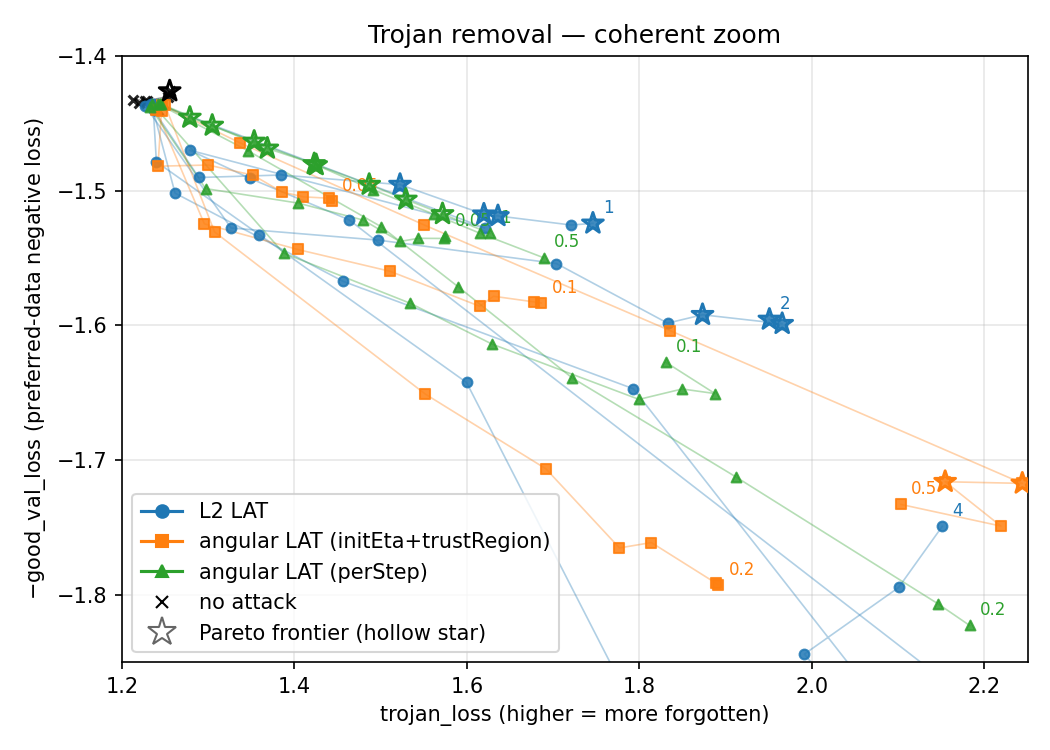
\includegraphics[width=\linewidth]{figures/synthesis/pareto_trojan_vs_good_zoom.png}
\caption{Trojan removal vs.\ capability across the coherent cells (Figure 4b convention of \citet{casper2024lat}). Each line is the 8-eval-step trajectory of one run; grey stars mark the union Pareto frontier. The full-range version, with the $L_2$ cliff at $\eps \in \{8, 16\}$ visible as a lower-right blob, is in Appendix~\ref{app:pareto-full}.}
\label{fig:pareto-synth}
\end{figure}

Figure~\ref{fig:pareto-synth} shows the Pareto curve across the coherent cells. Here are the main findings: 
\begin{itemize}[leftmargin=*]
\item \textbf{$L_2$ $\eps{=}1$ is the Pareto champion of the entire grid.} Exchange rate $6.07$; it dominates every angular cell at matched-or-lower $\Delta\text{good}$. The phase-1 result that ``RPGD owns the low-cost regime'' was an artefact of an undersampled $L_2$ grid (Casper's writeup never goes below $\eps{=}2$).
\item \textbf{The angular \texttt{perStep} curve is non-monotonic in $\thmax$.} $\Delta\text{good}$ and $\Delta\text{trojan}$ climb together from $\thmax{=}0.05$ to $\thmax{=}0.20$, then \emph{both} shrink at $\thmax{=}0.50$ and $\thmax{=}1.00$. This is not an $L_2$-style cliff (the model is not blown up): the adversary just stops using the budget productively. Figure~\ref{fig:trajectories} traces this on the eval-step axis: trojan loss peaks at $\thmax{=}0.20$ and is lower at both smaller and larger budgets, while good loss is similarly non-monotonic.
\item \textbf{\texttt{perStep} does not uniformly beat \texttt{initEta+TR}.} It wins at small $\thmax$ (e.g.\ $\thmax{=}0.20$: $+0.387/+0.941$ vs $+0.356/+0.641$) but loses at $\thmax{=}0.50$ ($+0.114/+0.445$ vs $+0.297/+0.857$). The best RPGD step rule is $\thmax$-dependent.
\end{itemize}

\begin{figure}[H]
\centering
\begin{subfigure}{0.49\textwidth}
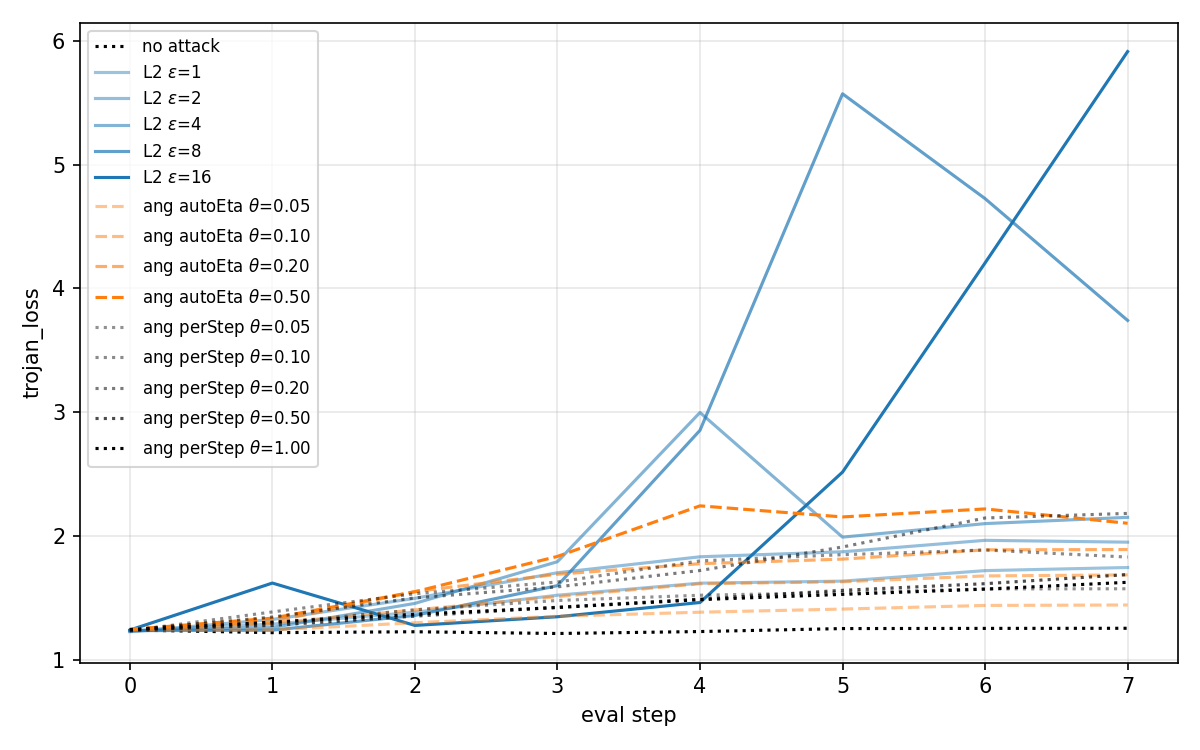
\includegraphics[width=\linewidth]{figures/synthesis/curve_trojan.png}
\caption{Trojan loss (higher $=$ more forgotten).}
\label{fig:curve-trojan}
\end{subfigure}\hfill
\begin{subfigure}{0.49\textwidth}
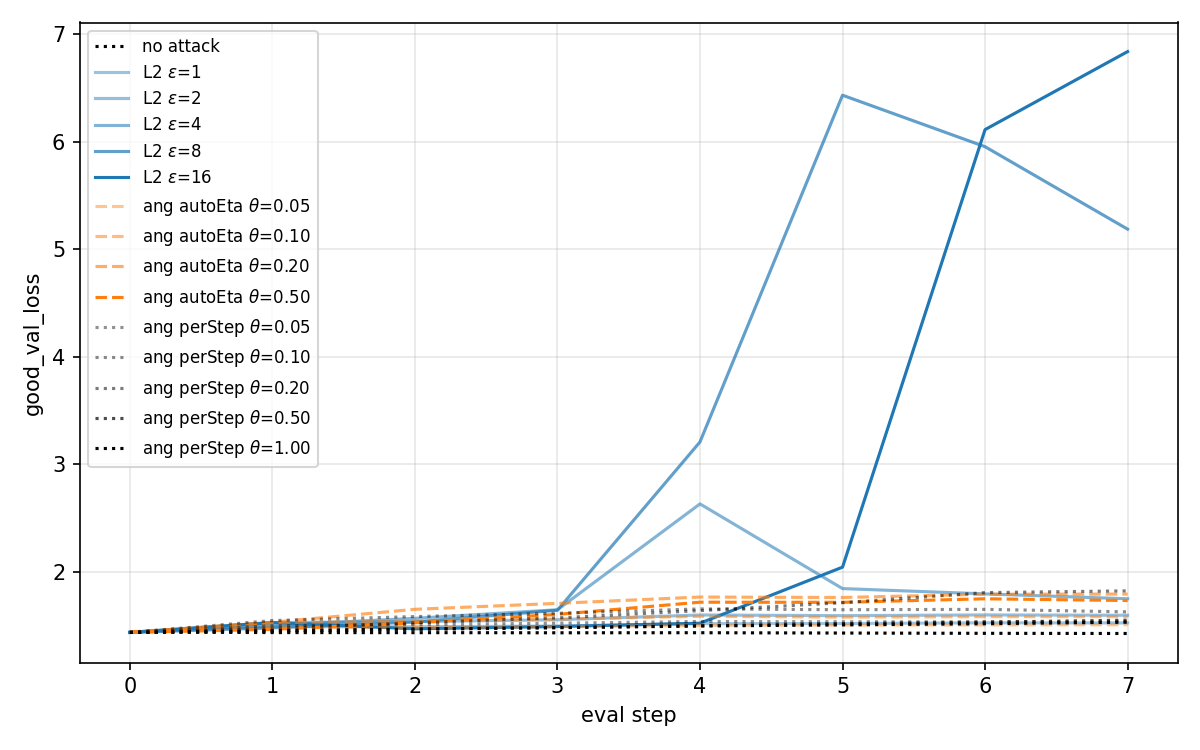
\includegraphics[width=\linewidth]{figures/synthesis/curve_good.png}
\caption{Preferred-data (good) loss (lower $=$ more capability retained).}
\label{fig:curve-good}
\end{subfigure}
\caption{Eval-step trajectories for each cell of the Phase~3 sweep (8 eval points per run). The angular \texttt{perStep} cells (curves labelled $\thmax \in \{0.05, 0.10, 0.20, 0.50, 1.00\}$) are non-monotonic in $\thmax$: $\thmax{=}0.20$ reaches the highest trojan loss while $\thmax \in \{0.50, 1.00\}$ both fall back, mirroring the behaviour on the good-loss axis.}
\label{fig:trajectories}
\end{figure}

Inner-loop diagnostics (Figure~\ref{fig:inner-perstep}) explain the fold-back. At $\thmax \le 0.20$ consecutive Riemannian gradients are well-aligned (cos-align $\approx 0.5{-}0.75$) and the inner loss climbs modestly; at $\thmax{=}0.50$ cos-align collapses to $\approx 0$ and the inner loss climbs to $\sim 17$ by $k = K{-}1$. The adversary is optimising hard in a regime where the per-step gradient signal becomes uncorrelated step-to-step. Per-step $\phi$ is flat at $\thmax/K$ for every cell by construction.

\begin{figure}[H]
\centering
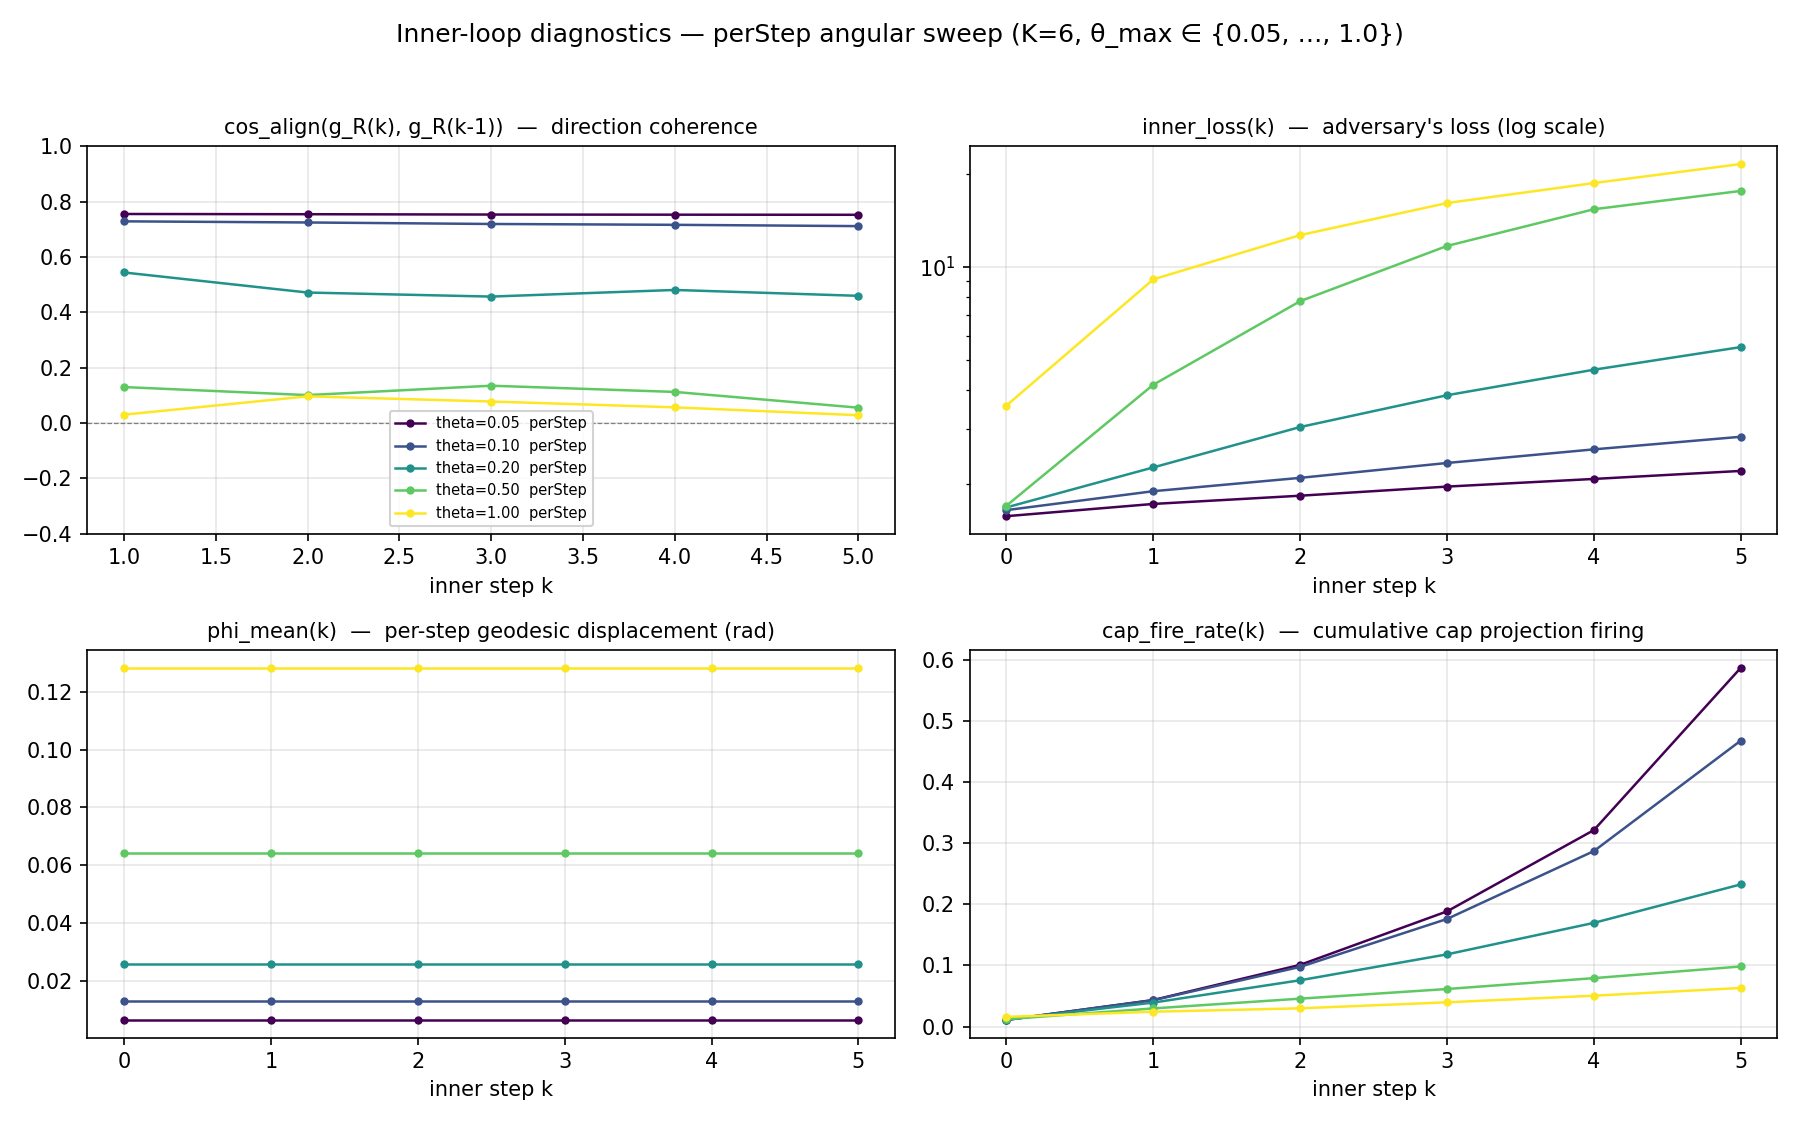
\includegraphics[width=0.95\linewidth]{figures/synthesis/inner_loop_perstep.png}
\caption{Per-step inner-loop diagnostics across the per-step-calib angular sweep at $K{=}6$. \texttt{cos\_align} (top-left): collapses toward $0$ at $\thmax \ge 0.50$. \texttt{inner\_loss} (top-right, log scale): grows much faster at larger $\thmax$ but doesn't translate into more $\Delta\text{trojan}$ outside. \texttt{phi\_mean} (bottom-left): flat at $\thmax/K$ for every cell as expected. \texttt{cap\_fire\_rate} (bottom-right): smaller $\thmax$ hits the cap more often, because coherent-direction inner steps accumulate towards the boundary in a straight line.}
\label{fig:inner-perstep}
\end{figure}

\FloatBarrier
\subsection{Phase 4: convergence study at $\thmax{=}0.50$, $K{=}24$}

It seems that \texttt{perStep} at $\thmax{=}0.50$ is optimising but not converging to a good solution within $K{=}6$ steps, and is folding back because the gradients become uncorrelated. There are two natural explanations. The first is that the per-step displacement is too large: raising $K$ so that $\thmax/K$ matches the coherent $\thmax{=}0.20/K{=}6$ value should recover coherence. The second is that the policy is wrong regardless of $K$: at large $\thmax$ the gradient signal degrades and the step rule should throttle when $\norm{g_R}$ shrinks, but \texttt{perStep} insists on $\thmax/K$ per step. To distinguish these we ran two cells at $\thmax{=}0.50$, $K{=}24$: cell A is \texttt{perStep} (matched per-step $\phi = 0.021$ rad to the coherent baseline), cell B is \texttt{fixed} with $\eta{=}0.5$.

\begin{table}[h]
\centering\small
\begin{tabular}{lcccc}
\toprule
\textbf{cell} & $\Delta\text{good}\downarrow$ & $\Delta\text{trojan}\uparrow$ & $\Delta\text{t}/\Delta\text{g}$ & cos-align$_{K{-}1}$ \\
\midrule
\texttt{initEta+TR}, $K{=}6$, $\thmax{=}0.50$ (anchor) & $+0.297$ & $+0.857$ & $2.89$ & --- \\
\texttt{perStep}, $K{=}6$, $\thmax{=}0.50$            & $+0.114$ & $+0.445$ & $3.90$ & $+0.056$ \\
\textbf{A: \texttt{perStep}, $K{=}24$, $\thmax{=}0.50$}        & $+0.126$ & $+0.414$ & $3.28$ & $\mathbf{-0.296}$ \\
\textbf{B: \texttt{fixed}, $\eta{=}0.5$, $K{=}24$}             & $+0.322$ & $+0.725$ & $2.25$ & $+0.264$ \\
\bottomrule
\end{tabular}
\end{table}

Figure~\ref{fig:inner-k24} shows the inner-loop diagnostics for the two $K{=}24$ cells, overlaid with the $K{=}6$ baselines for context.
\begin{itemize}[leftmargin=*]
\item \textbf{The first hypothesis is falsified.} At matched per-step $\phi$, \texttt{perStep} at $K{=}24$ still folds back ($\Delta\text{good}/\Delta\text{trojan}$ essentially identical to $K{=}6$). cos-align does more than drop; it goes \emph{negative} ($-0.30$), meaning the adversary is oscillating (step, gradient flips $\sim 180^\circ$, step back). Per-step displacement alone is not the determinant; trajectory length to the chaotic region is.
\item \textbf{The second is partially confirmed.} \texttt{fixed} at $K{=}24$ keeps cos-align positive throughout and takes adaptively-sized steps (per-step $\phi$ grows with $\norm{g_R}$ from $0.007$ to $0.049$), recovering most of the $K{=}6$ \texttt{initEta+TR} survivor: $\Delta\text{good}$ matches, $\Delta\text{trojan}$ is $\sim 85\%$. Gradient-magnitude-aware sizing is the right policy at large $\thmax$, but no tested configuration beats the $K{=}6$ ceiling.
\end{itemize}

\begin{figure}[H]
\centering
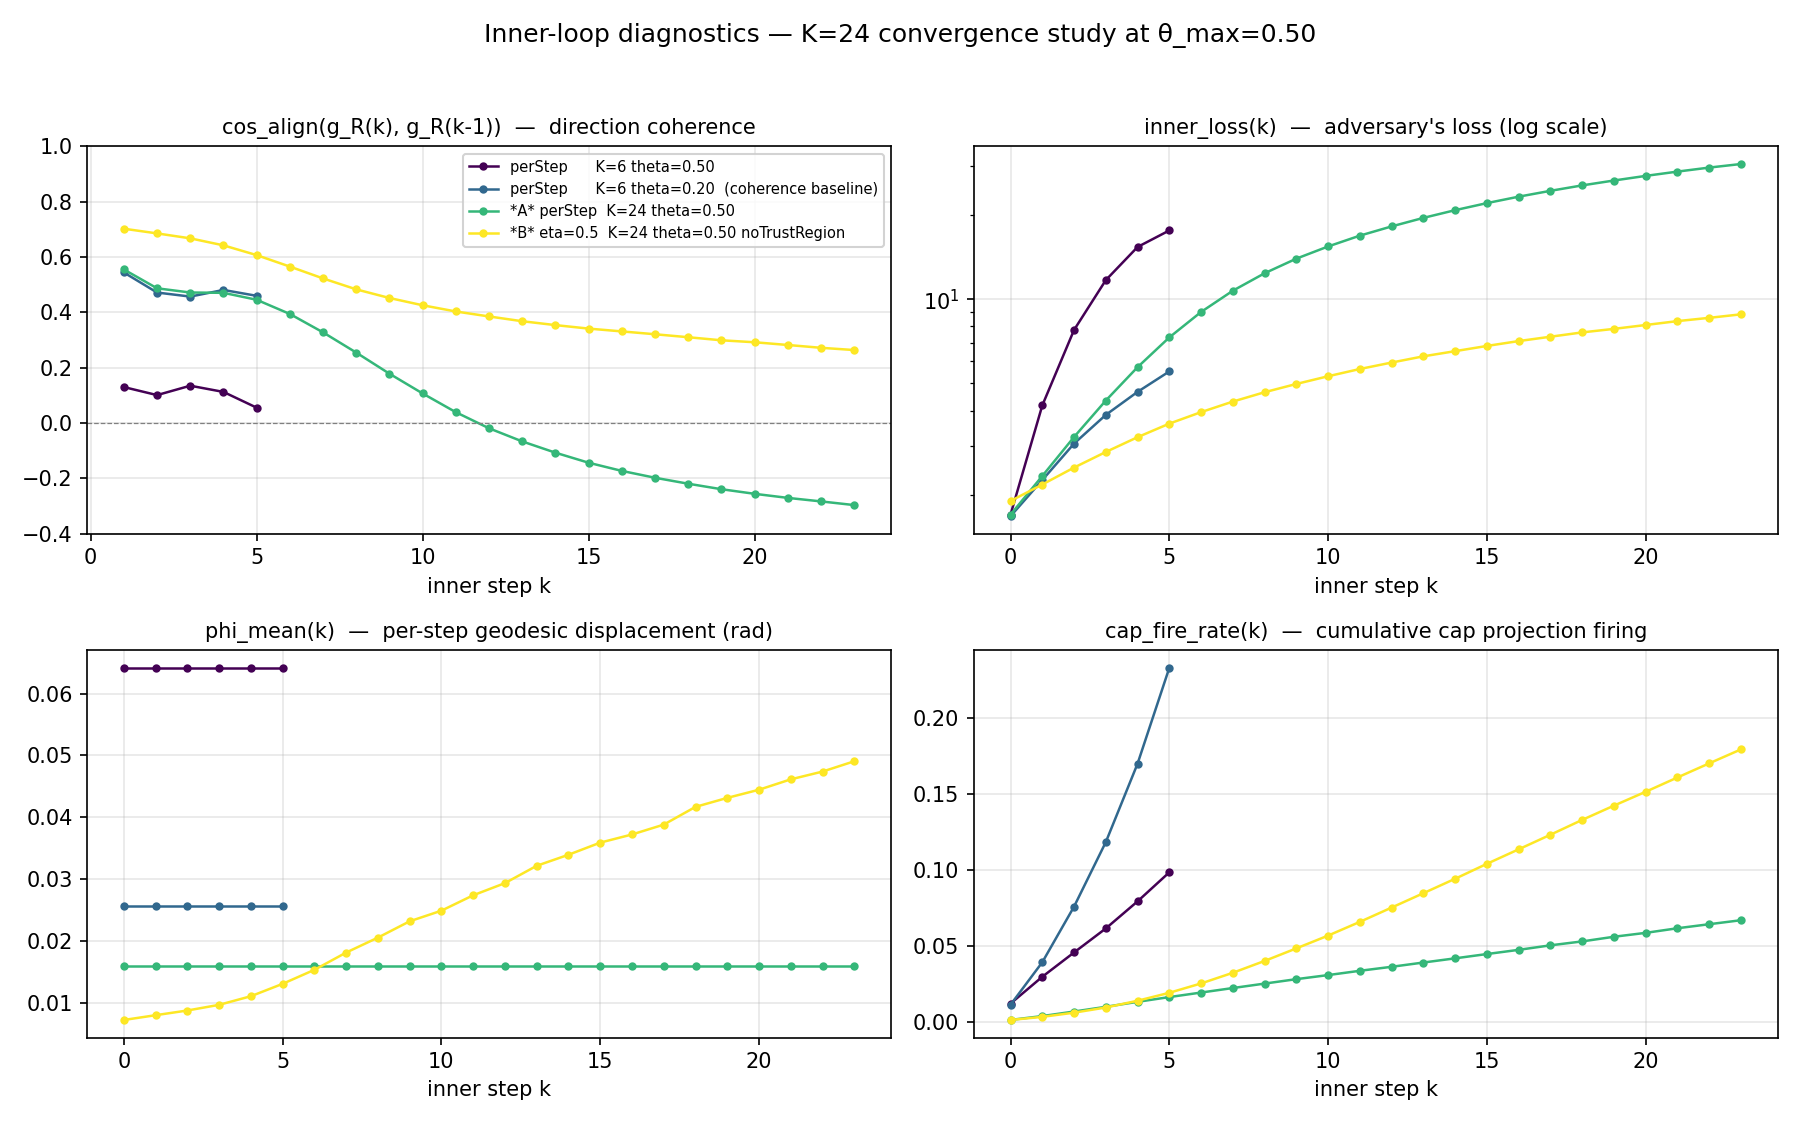
\includegraphics[width=0.95\linewidth]{figures/synthesis/inner_loop_k24.png}
\caption{Inner-loop diagnostics at $\thmax{=}0.50$ with $K{=}24$, with the $K{=}6$ cells overlaid (cells in $\thmax{=}0.50$ and the coherent $\thmax{=}0.20$ baseline). Cell A (perStep $K{=}24$) decays through zero around $k{=}12$ and reaches $-0.30$ at $k{=}23$; Cell B (fixed $\eta{=}0.5$, $K{=}24$) stays positive throughout.}
\label{fig:inner-k24}
\end{figure}

\FloatBarrier
\subsection{Take-aways}

\begin{itemize}[leftmargin=*]
\item \textbf{$L_2$ $\eps \in \{1, 2, 4\}$ owns the coherent Pareto frontier} on TinyLlama-1.1B at layer 4. $\eps{=}1$ dominates the low-cost end ($\Delta\text{good} \approx 0.08$); $\eps \in \{2, 4\}$ dominate the moderate-cost band ($\Delta\text{good} \approx 0.15{-}0.30$).
\item \textbf{Angular has no $L_2$-style cliff but does have an intrinsic ceiling} at $\Delta\text{trojan} \approx +0.85{-}+0.94$ that no tested step policy extends. The cliff regime for $L_2$ ($\eps \ge 8$) is unreachable by the angular method by construction.
\item \textbf{The canonical RPGD step rule is $\thmax$-dependent}, not single-mode. \texttt{perStep} at small $\thmax$ ($\le 0.20$); \texttt{initEta+TR} at large $\thmax$ ($= 0.50$).
\item In general, the results across the two methods are qualitatively similar, with RPGD possibly making the optimisation process more difficult.
\item \textbf{Geometric note: why $L_2$ and angular cluster.} The perturbation is injected into the residual stream \emph{before} layer 4's RMSNorm, which satisfies $\text{RMSNorm}(\alpha x) = \text{RMSNorm}(x)$ for $\alpha > 0$. Layer 4's attention output has zero first-order sensitivity to the radial component of any perturbation, so $L_2$ and angular both have to leverage the dominant tangent direction. $L_2$ additionally has access to the radial direction via residual-stream propagation into downstream layers, which empirically is less useful but not zero. The clustering of $L_2$ and angular cells on the same Pareto ridge is consistent with both methods mostly exploiting the same tangent direction; the methods are probably $\sim$equivalent at this site, with angular possibly a slightly harder optimisation problem and the radial channel giving $L_2$ a small additional handle. 
\end{itemize}

\section{Discussion and next steps}

\paragraph{Improving convergence.}
The adversary's optimisation still doesn't behave perfectly, and there remain a few knobs we could turn, inlcuding the learning rate schedule, number of inner steps (and alternating training), as well as parameter efficient fine-tuning (which aside from drastically reducing our iteration speed, might give regularisation benefits).
I don't expect any of these to preferentially impact our method though, so these seem like general improvements to the overall LAT framework, independent of the spherical geometry. 

\paragraph{Relaxing Spherical cap to include a radial component (turn it into a cone)}


\paragraph{Looking at realistic evaluation performance.}
All of the above methods and configurations are evaluated based on the trojan-loss. This relies on the assumption of this being a good proxy for general adversarial robustness. This might not be true, or more generally the proxy might not be very precise. 
Evaluating against realistic downstream adversarial robustness would 


\paragraph{Other perturbation sites (partly done).}
Given note on the geometry of the perturbation sites above, it would be interesting to test these methods at sites where the radial direction is not ablated by layer normalisation. 
Unfortunately, initial experiments on the internal attention outputs (`queries' in this case) show that performance is more or less identical even here, after some hyperparameter tuning for both methods.


\paragraph{Soft-prompt adversarial training.}
Instead of optimising against a worst-case perturbation in the representation space (of any geometry) we could optimise against a soft-prompt adversary in the `soft-input' space. 


\paragraph{Attack geometry study.}
As discussed previously, we could drop the 'unforseen attacker' requirement and study the representation geometry for successful adversarial attacks and jailbreaks, and tune our approach accordingly.


\bibliographystyle{plainnat}
\bibliography{references}

\appendix

\section{Equivalence with the Slerp reformulation}
\label{app:riemannian}

The body of \S\ref{sec:projection} states the Riemannian PGD inner loop in exp-map form: tangent project, geodesic step via $\exp_{h_k}$, Slerp projection onto the cap boundary when needed. We collect here a parallel presentation that uses the same spherical linear interpolation primitive that \citet{you2026spherical} use for inference-time directional steering, and show that the two presentations describe the same algorithm. The point is twofold: (i) make the connection to the steering literature explicit, since the Slerp operation appears verbatim there; (ii) keep the core algorithm self-contained at textbook level for readers approaching from the Riemannian-optimisation side.

\subsection*{Riemannian PGD on the spherical cap: full formalisation}

For reference, we restate the Riemannian-PGD construction of \S\ref{sec:projection} with a slightly more textbook framing. The material (manifold and tangent space, Riemannian gradient as ambient projection, closed-form exponential map on the sphere, geodesic projection onto the cap) is standard differential geometry; for a self-contained treatment of Riemannian optimisation we point to \citet{boumal2023introduction}, and for the stochastic-gradient analysis on manifolds see \citet{bonnabel2013stochastic, tripuraneni2018averaging}.

\paragraph{Manifold and tangent space.} Let $r = \norm{h_0}$. The constraint manifold is the sphere of radius $r$ centred at the origin,
\begin{equation*}
\mathcal{M} \;=\; \mathcal{S}^{d-1}(r) \;=\; \big\{ h \in \R^d : \norm{h}_2 = r \big\}.
\end{equation*}
At any $h \in \mathcal{M}$, the tangent space is the linear subspace orthogonal to $h$,
\begin{equation*}
T_h \mathcal{M} \;=\; \big\{ v \in \R^d : h^\top v = 0 \big\},
\end{equation*}
of dimension $d-1$.

\paragraph{Riemannian metric and gradient.} We use the Riemannian metric induced from the ambient Euclidean inner product: for $u, v \in T_h \mathcal{M}$, $\inner{u}{v}_h = u^\top v$. The Riemannian gradient at $h$ is the orthogonal projection of the ambient Euclidean gradient onto the tangent space:
\begin{equation}
\mathrm{grad}_{\mathcal{M}}\,\mathcal{L}(h) \;=\; \big(I - \hh\,\hh^\top\big)\,\nabla_{\R^d}\mathcal{L}(h), \qquad \hh = h/\norm{h}.
\end{equation}
The matrix $\hh\,\hh^\top$ is the rank-one orthogonal projector onto the line through $h$, and $I - \hh\,\hh^\top$ is the projector onto $T_h \mathcal{M}$.

\paragraph{Exponential map.} The exponential map at $h$ moves a point along the geodesic emanating from $h$ in the direction of a tangent vector $v \in T_h\mathcal{M}$, by an arc length equal to $\norm{v}$. On $\mathcal{M} = \mathcal{S}^{d-1}(r)$, geodesics are great circles, and the exponential has the closed form
\begin{equation}
\exp_h(v) \;=\; \cos\!\Big(\frac{\norm{v}}{r}\Big)\,h \;+\; \sin\!\Big(\frac{\norm{v}}{r}\Big)\,r\,\frac{v}{\norm{v}}.
\end{equation}
The argument $\norm{v}/r$ is the angle subtended at the origin: a tangent step of Euclidean length $\norm{v}$ on a sphere of radius $r$ traces an arc of $\norm{v}/r$ radians. For the unit sphere ($r = 1$) this collapses to $\exp_h(v) = \cos(\norm{v})\,h + \sin(\norm{v})\,v/\norm{v}$.

\paragraph{Constraint set: the spherical cap.} The angular constraint $\angle(h, h_0) \le \thmax$ defines a spherical cap on $\mathcal{M}$,
\begin{equation*}
\mathcal{C} \;=\; \{ h \in \mathcal{M} : \hh_0^\top \hh \ge \cos\thmax \},
\end{equation*}
whose boundary $\partial\mathcal{C}$ is the set of points exactly $\thmax$ radians from $h_0$. Geometrically, $\partial\mathcal{C}$ is the intersection of $\mathcal{M}$ with the affine hyperplane $\hh_0^\top \hh = \cos\thmax$. Unless $\thmax = \pi/2$, this hyperplane does not pass through the origin, so $\partial\mathcal{C}$ is a \emph{small circle}: a $(d-2)$-sphere of radius $r\sin\thmax$ centred at the point $r\cos\thmax\,\hh_0$, lying in a hyperplane parallel to but offset from the equatorial one through the origin.

\paragraph{Why projection by Slerp from $\hh_0$, not by tangent stepping along $\partial\mathcal{C}$.} Geodesics on $\mathcal{M}$ are great circles, which are intersections of $\mathcal{M}$ with hyperplanes \emph{through} the origin. Small circles and great circles do not coincide except at $\thmax = \pi/2$ (the equator), so the boundary $\partial\mathcal{C}$ is not itself a geodesic of $\mathcal{M}$. A consequence: a tangent step from a point on $\partial\mathcal{C}$ taken along the direction tangent to the small circle still leaves $\partial\mathcal{C}$, because the geodesic curves into $\mathcal{C}$'s interior or exterior rather than tracing the small circle. The standard correction is the metric (geodesic) projection: take the great circle through $\hh_0$ and the candidate iterate, and stop at the intersection with $\partial\mathcal{C}$. This is exactly what spherical linear interpolation between $\hh_0$ and the candidate computes when its parameter is set to $\thmax/\alpha$, where $\alpha$ is the candidate's angle from $\hh_0$.

\paragraph{Algorithm.} Putting the ingredients together, RPGD on the cap is exactly Algorithm~\ref{alg:rpgd} in \S\ref{sec:rpgd-impl}. The cap projection (line~16 there) is Slerp$(\hh_0, h^*/r;\, t = \thmax/\alpha)$: parameter $t$ is set so that the interpolated angle from $\hh_0$ equals $\thmax$, that is, $t\alpha = \thmax$. Substituting into the standard Slerp formula gives the projection expression. The choice of step size $\eta$ is left to the user; the standard RPGD analysis covers both fixed $\eta$ and decreasing schedules \citep{bonnabel2013stochastic, tripuraneni2018averaging}.

\subsection*{A Slerp reformulation with moving reference}

The directional steering literature \citep{you2026spherical} parameterises an activation rotation as a spherical linear interpolation \citep{shoemake1985slerp} between two unit vectors: the current direction $\hh = h/\norm{h}$ and a target direction $\mu_T \in S^{d-1}$. For a fraction $t \in [0,1]$, with $\theta = \arccos(\hh^\top \mu_T)$,
\begin{equation*}
\hh' \;=\; \frac{\sin((1-t)\theta)}{\sin\theta}\,\hh \;+\; \frac{\sin(t\theta)}{\sin\theta}\,\mu_T,
\end{equation*}
and the perturbed activation is $h' = \norm{h}\,\hh'$. The geometry is a movement of $\hh$ toward $\mu_T$ along the great circle through them, by a fraction $t$ of the angle $\theta$ separating them. \citet{you2026spherical} use this primitive once at inference time, with $\mu_T$ a precomputed contrastive prototype. Here we adapt it to the inner-loop adversary by re-applying it $K$ times with a \emph{moving} reference: at iteration $k$, given the current iterate $h_k$ (with $h_0$ the unperturbed activation), pick a target $\mu_{T,k}$ and a fraction $t_k$, set
\begin{equation*}
h_{k+1} \;=\; \norm{h_0} \cdot \mathrm{Slerp}\!\left(\hh_k,\, \mu_{T,k},\, t_k\right),
\end{equation*}
and re-evaluate the model gradient at $h_{k+1}$ to choose $(\mu_{T,k+1}, t_{k+1})$ for the next step. The reference direction $\hh_k$ is updated each iteration; only the original norm $\norm{h_0}$ is retained, so the iterate stays on the sphere of radius $\norm{h_0}$ throughout.

Two natural choices of $\mu_{T,k}$ make the scheme operational. Let $g_{\perp,k} = \nabla_h \mathcal L(h_k) - \inner{\hh_k}{\nabla_h \mathcal L(h_k)}\,\hh_k$ be the tangent gradient at $h_k$, and $\hat g_{\perp,k} = g_{\perp,k}/\norm{g_{\perp,k}}$ its unit-normalised form.

\begin{itemize}[leftmargin=*]
\item \textbf{Tangent target.} Set $\mu_{T,k} = \hat g_{\perp,k}$. Since $\hat g_{\perp,k} \perp \hh_k$ we have $\theta_k = \pi/2$, and the Slerp simplifies to
\begin{equation*}
\hh_{k+1} \;=\; \cos(t_k\pi/2)\,\hh_k \;+\; \sin(t_k\pi/2)\,\hat g_{\perp,k}.
\end{equation*}
The cap constraint $\angle(h_0, h_{k+1}) \le \thmax$ becomes a coupled bound on the cumulative angle stepped, $\sum_k t_k \pi/2 \le \thmax$.
\item \textbf{Boundary target.} Set $\mu_{T,k} = \cos(\thmax)\,\hh_k + \sin(\thmax)\,\hat g_{\perp,k}$. This unit vector lies in the plane spanned by $\hh_k$ and $\hat g_{\perp,k}$, at angle $\thmax$ from $\hh_k$ (note: from the \emph{current} $\hh_k$, not from $\hh_0$). Then $\theta_k = \thmax$ and $t_k \in [0,1]$ maps directly to a \emph{per-step} angular displacement in $[0, \thmax]$. The bound $t_k \le 1$ controls only the per-step step size; the cap constraint $\angle(h_0, h_{k+1}) \le \thmax$ is a constraint on the cumulative angle from $\hh_0$ over all $k$ and is not implied by $t_k \le 1$. We enforce it explicitly via a Slerp projection from $\hh_0$ as described below.
\end{itemize}

Either choice gives a complete inner-loop algorithm: a single Slerp call from the current iterate replaces the exp-map step of Algorithm~\ref{alg:rpgd}, with the cumulative angle clipped against $\hh_0$ if it exceeds $\thmax$.

\subsection*{Detailed equivalence between the Slerp reformulation and Riemannian PGD}

We now show in detail that the moving-reference Slerp scheme and Algorithm~\ref{alg:rpgd} (RPGD) produce identical iterate sequences. The argument has three pieces: the per-step inner update, the cap projection, and the step-size correspondence. Each piece is a closed-form identity; assembled, they give an iterate-by-iterate identity.

\paragraph{Setup.} Both algorithms take as input the same data: an initial activation $h_0 \in \R^d$ defining the sphere $\mathcal{M} = \mathcal{S}^{d-1}(r)$ with $r = \norm{h_0}$ and the cap $\mathcal{C} = \{h \in \mathcal{M} : \angle(h_0, h) \le \thmax\}$, a loss $\mathcal{L}: \R^d \to \R$, and a step count $K$. At iteration $k$ both algorithms have a current iterate $h_k \in \mathcal{C}$ and compute the same Riemannian gradient $g_{R,k} = (I - \hh_k\hh_k^\top)\,\nabla_h\mathcal{L}(h_k)$ with unit form $\hat g_{\perp,k} = g_{R,k}/\norm{g_{R,k}}$ (assuming $g_{R,k} \neq 0$). What differs is how the next iterate is constructed from these quantities. We show the constructions yield the same point.

\paragraph{Step 1: per-step update is identical (Slerp = exp map).} The RPGD per-step candidate is the exponential map evaluated at $v = \eta\,g_{R,k}$, that is
\begin{equation}
h_{k+1}^{\,\text{RPGD}} \;=\; \exp_{h_k}(\eta\,g_{R,k}) \;=\; \cos\!\Big(\frac{\eta\,\norm{g_{R,k}}}{r}\Big)\,h_k \;+\; \sin\!\Big(\frac{\eta\,\norm{g_{R,k}}}{r}\Big)\,r\,\hat g_{\perp,k}.
\label{eq:rpgd-step}
\end{equation}
The boundary-target Slerp candidate is, by definition,
\begin{equation*}
h_{k+1}^{\,\text{Slerp}} \;=\; r\,\mathrm{Slerp}(\hh_k,\, \mu_{T,k},\, t_k), \qquad \mu_{T,k} = \cos\thmax\,\hh_k + \sin\thmax\,\hat g_{\perp,k}.
\end{equation*}
Expand the Slerp using $\theta_k = \arccos(\hh_k^\top \mu_{T,k}) = \thmax$ (since $\hh_k^\top \mu_{T,k} = \cos\thmax$):
\begin{equation*}
\mathrm{Slerp}(\hh_k,\, \mu_{T,k},\, t_k) \;=\; \frac{\sin\!\big((1-t_k)\thmax\big)}{\sin\thmax}\,\hh_k \;+\; \frac{\sin(t_k\thmax)}{\sin\thmax}\,\mu_{T,k}.
\end{equation*}
Substitute the expression for $\mu_{T,k}$:
\begin{align*}
&= \frac{\sin\!\big((1-t_k)\thmax\big)}{\sin\thmax}\,\hh_k + \frac{\sin(t_k\thmax)}{\sin\thmax}\,\big[\cos\thmax\,\hh_k + \sin\thmax\,\hat g_{\perp,k}\big]\\
&= \underbrace{\frac{\sin\!\big((1-t_k)\thmax\big) + \sin(t_k\thmax)\cos\thmax}{\sin\thmax}}_{\text{coefficient of }\hh_k}\,\hh_k \;+\; \sin(t_k\thmax)\,\hat g_{\perp,k}.
\end{align*}
Apply the angle-subtraction identity to the numerator of the $\hh_k$ coefficient:
\begin{align*}
\sin\!\big((1-t_k)\thmax\big) &= \sin\thmax\cos(t_k\thmax) - \cos\thmax\sin(t_k\thmax),
\end{align*}
hence
\begin{equation*}
\sin\!\big((1-t_k)\thmax\big) + \sin(t_k\thmax)\cos\thmax \;=\; \sin\thmax\cos(t_k\thmax),
\end{equation*}
and the coefficient of $\hh_k$ collapses to $\cos(t_k\thmax)$. Combining,
\begin{equation*}
\mathrm{Slerp}(\hh_k,\, \mu_{T,k},\, t_k) \;=\; \cos(t_k\thmax)\,\hh_k + \sin(t_k\thmax)\,\hat g_{\perp,k}.
\end{equation*}
Multiplying through by $r$ gives the boundary-target Slerp candidate
\begin{equation}
h_{k+1}^{\,\text{Slerp}} \;=\; \cos(t_k\thmax)\,h_k \;+\; \sin(t_k\thmax)\,r\,\hat g_{\perp,k}.
\label{eq:slerp-step}
\end{equation}
Compare \eqref{eq:slerp-step} with \eqref{eq:rpgd-step}: the two candidates coincide as functions of $h_k$ and $\hat g_{\perp,k}$ if and only if their angular arguments are equal,
\begin{equation}
t_k\,\thmax \;=\; \frac{\eta\,\norm{g_{R,k}}}{r} \quad\Longleftrightarrow\quad t_k \;=\; \frac{\eta\,\norm{g_{R,k}}}{r\,\thmax}.
\label{eq:tk-eta}
\end{equation}
This is a one-line algebraic identity; nothing else need be checked. The geometric reason is that both expressions parameterise the same geodesic on $\mathcal{M}$ (the great circle in the plane spanned by $\hh_k$ and $\hat g_{\perp,k}$) by the same arc-length, just with two different naming conventions for the arc-length itself.

The tangent-target variant ($\mu_{T,k} = \hat g_{\perp,k}$, so $\theta_k = \pi/2$) yields by the same computation
\begin{equation*}
h_{k+1}^{\,\text{Slerp,tan}} \;=\; \cos(t_k\pi/2)\,h_k + \sin(t_k\pi/2)\,r\,\hat g_{\perp,k},
\end{equation*}
which matches \eqref{eq:rpgd-step} under $t_k\,\pi/2 = \eta\norm{g_{R,k}}/r$, i.e.\ $t_k = 2\eta\norm{g_{R,k}}/(\pi r)$. So both Slerp variants are equivalent to RPGD; only the meaning of the scalar $t_k$ differs.

\paragraph{Step 2: cap projection is identical.} If the per-step candidate $h_{k+1}^*$ (whichever symbol) lies inside $\mathcal{C}$, both algorithms accept it as $h_{k+1}$. If $h_{k+1}^*$ lies outside, both algorithms project to the boundary along the great circle from $\hh_0$:
\begin{equation*}
\hh_{k+1} \;=\; \frac{\sin(\alpha - \thmax)}{\sin\alpha}\,\hh_0 \;+\; \frac{\sin\thmax}{\sin\alpha}\,\hh_{k+1}^*, \qquad \alpha = \angle(\hh_0, \hh_{k+1}^*).
\end{equation*}
This is Slerp$(\hh_0, \hh_{k+1}^*;\, t = \thmax/\alpha)$, the metric projection onto $\partial\mathcal{C}$. It is the same line of code in both algorithms (Algorithm~\ref{alg:rpgd}, line~16). No derivation is required for this piece; both algorithms simply call the same projection routine.

\paragraph{Step 3: step-size correspondence and matched schedules.} Equation~\eqref{eq:tk-eta} translates one knob into the other but does \emph{not} fix a step-size schedule. Both algorithms admit any schedule of $\eta_k$ or $t_k$; matched comparison requires choosing schedules that satisfy \eqref{eq:tk-eta} per iteration. Two natural matched conventions:
\begin{itemize}[leftmargin=*]
\item \textbf{Constant $\eta$.} The angular step $\eta\norm{g_{R,k}}/r$ varies with the gradient magnitude: large gradients produce large steps. Translating to Slerp, $t_k = \eta\norm{g_{R,k}}/(r\thmax)$ is a state-dependent fraction. This is the standard Riemannian SGD/SGM convention, the one analysed in \citet{bonnabel2013stochastic, tripuraneni2018averaging}.
\item \textbf{Constant angular step $t_k\thmax = \thmax/K$.} The angular displacement is fixed at $\thmax/K$ per iteration, so $K$ aligned steps exactly cover the budget. Translating to RPGD, $\eta_k = r\thmax/(K\norm{g_{R,k}})$ varies inversely with the gradient magnitude. This is the per-step-calibration mode of \S\ref{sec:rpgd-impl} and is the gradient-normalised analogue of standard $L_p$-ball PGD.
\end{itemize}
Different schedules give different iterate sequences, but both algorithms admit either schedule. The equivalence \eqref{eq:tk-eta} is a per-iteration identity, not a schedule-dependent claim.

\paragraph{Iterate-by-iterate identity.} Combining the three pieces: starting from the same $h_0 \in \mathcal{C}$ and presented with the same sequence of ambient gradients $\nabla\mathcal{L}(h_0), \nabla\mathcal{L}(h_1), \dots$, with $\eta_k$ and $t_k$ matched per~\eqref{eq:tk-eta}, the two algorithms produce the same iterate $h_k$ at every $k$. Inductively: $h_0$ matches by definition; if $h_k$ matches in both algorithms then so does $g_{R,k}$ (it is determined by $h_k$ and $\mathcal{L}$); the per-step candidate $h_{k+1}^*$ matches by step~1 above; the cap projection (if triggered) matches by step~2; therefore $h_{k+1}$ matches. The two algorithms have the same fixed points, the same convergence rates, the same stability and stationarity conditions, and the same dependence on the curvature and topology of $\mathcal{C}$.

\paragraph{What the two presentations buy us.} The exp-map presentation (the one used in the main body, \S\ref{sec:projection}) makes the convergence theory directly cite-able from the Riemannian-optimisation literature \citep{bonnabel2013stochastic, tripuraneni2018averaging, boumal2023introduction} and is the more economical implementation: one ambient gradient, one tangent project, one exp map, one conditional Slerp. The Slerp-reformulation presentation makes the operational connection to inference-time directional steering \citep{you2026spherical} explicit: the same closed-form rotation primitive that they apply once with a precomputed $\mu_T$ is here applied $K$ times with a moving reference. They are the same algorithm.

\section{Full-range Pareto plot}
\label{app:pareto-full}

The full-range counterpart to Figure~\ref{fig:pareto-synth}, including the $L_2$ cliff cells at $\eps \in \{8, 16\}$ that collapse the model.

\begin{figure}[h]
\centering
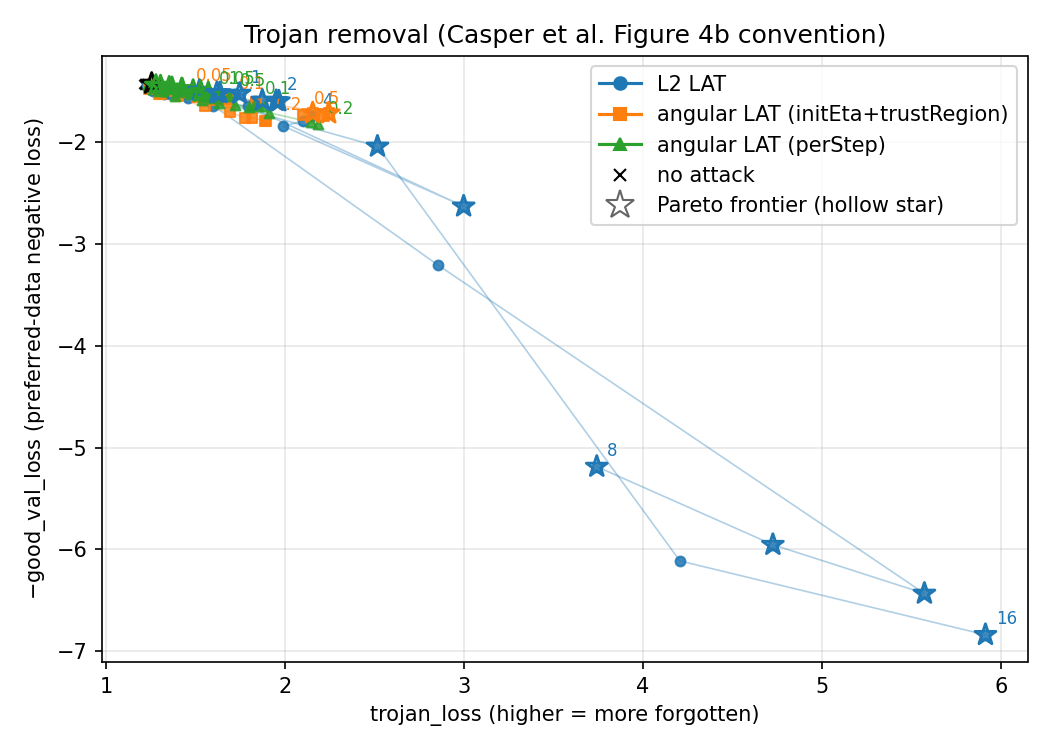
\includegraphics[width=\linewidth]{figures/synthesis/pareto_trojan_vs_good.png}
\caption{Trojan removal vs.\ capability across all cells. The lower-right blob is the $L_2$ cliff at $\eps \in \{8, 16\}$: technically Pareto-undominated because broken models score high on trojan loss, but unusable. The meaningful comparison lives in the upper-left cluster shown zoomed in Figure~\ref{fig:pareto-synth}.}
\label{fig:pareto-full}
\end{figure}

\section{Hyperparameters and compute}
\label{app:hyperparams}

Held-fixed hyperparameters across all runs:

\begin{table}[h]
\centering
\small
\begin{tabular}{l l p{0.27\textwidth}}
\toprule
& \textbf{Setting} & \textbf{Source} \\
\midrule
Backbone & Llama-2-7b-chat (fp32, no mixed precision) & Casper \\
Optimiser & AdamW, $\text{lr} = 5\!\times\!10^{-6}$, weight decay $6\!\times\!10^{-4}$ & Casper \\
LR schedule & constant, 3\% warmup & Casper \\
Effective batch size & 64 (per-device 4, grad-accum 16) & ours; Casper used 8/8 (per-device halved to fit memory under PGD's retained-graph buffer accumulation) \\
Max sequence length & 512 & Casper \\
Gradient clipping & max-norm $0.25$ & Casper \\
Epochs & 1 (each phase) & Casper \\
PGD steps $K$ & 6 & Casper \\
Step size & $\eps / K$ ($L_2$) or $\thmax / K$ (angular) & ours, mirroring Casper's $L_2$ rule \\
Random init & yes (uniform in ball / cap) & Casper default \\
Perturbation site & residuals, layer 4 (of 32) & Casper §4.3 \\
Eval frequency & every $1/8$ of training (8 evals/run) & Casper default \\
\bottomrule
\end{tabular}
\caption{Held-fixed hyperparameters for both phases and both methods. Rows marked ``Casper'' inherit the value from \citet{casper2024lat}.}
\label{tab:hyperparams}
\end{table}

The two phase-1 budgets in the preliminary run are $L_2$ with $\eps = 8$ and angular with $\thmax = 0.20$ radians ($\approx 11.5^\circ$).

\paragraph{Compute.} Each phase 1 run takes $\sim 70$\,min on $4 \times$ A100-80GB. The two phase-1 runs were launched in parallel. Total wall clock for the preliminary experiment was approximately 2\,h\,17\,min for Phase 1; Phase 0 was inherited from a previous run.

\end{document}
